\documentclass[12pt,a4paper]{article}

\usepackage[utf8]{inputenc}
\usepackage{ctex}
\usepackage{amsmath,amsfonts,amssymb}
\usepackage{abstract,appendix}
\usepackage{makeidx,hyperref}
\usepackage{graphicx,epsfig,subfig}
\usepackage{geometry}
\usepackage{color,xcolor}
\usepackage{listings}

\lstset{
basicstyle=\footnotesize,                  % 设定代码字体
backgroundcolor=\color[RGB]{239,239,239},  % 设定背景颜色
keywordstyle=\color[RGB]{40,40,255},       % 设定关键字颜色
commentstyle=\color[RGB]{0,96,96},         % 设置代码注释的格式
stringstyle=\color[RGB]{128,0,0},          % 设置字符串格式
language=python,                           % 设置语言
}

\geometry{scale=0.8}

%\setlength{\lineskip}{\baselineskip}
\setlength{\parskip}{0.5\baselineskip}

\title{深度学习(Mscale网络)求解椭圆方程代码模板(Deep-Ritz方法)}
\author{sis-flag}
\date{\today}

\begin{document}

\maketitle

根据神经网络的F-principle,网络在训练的过程中会优先拟合训练数据的低频部分。但是在某些特殊的场合下(如使用神经网络求解微分方程),需要拟合目标函数的高频部分。实验希望找到一种特殊的网络结构,更快地拟合目标函数的高频部分。

这里提出了一种新的网络结构:Mscale,用于求解椭圆方程。

\section*{椭圆方程的Ritz方法}

椭圆方程的一般形式为
\begin{align*}
-\nabla(a(x) \nabla u(x)) + c(x) u(x) = f(x) \quad x \in \Omega \\
u(x) = u_0(x) \quad x \in \partial \Omega
\end{align*}

通过数学上的推导\cite{deep-ritz},方程可以转化为泛函的极小值问题
\begin{align*}
\min_{u} J(u) & = \int_{\Omega} \frac{1}{2} a(x) |\nabla u(x)|^2 + c(x) |u(x)|^2 - f(x) u(x) \ dx \\
\text{s.t.} \quad u(x) & = u_0(x) \quad x \in \partial \Omega 
\end{align*}

这是一个约束优化问题,我们用加惩罚项的方法把它近似转化成无约束优化问题
\begin{align*}
\min_{u} \int_{\Omega} \frac{1}{2} a(x) |\nabla u(x)|^2 + \frac{1}{2} c(x) |u(x)|^2 - f(x) u(x) \ dx + \int_{\partial \Omega} |u(x) - u_0(x)|^2 \ dx
\end{align*}

用神经网络$N(x; \theta)$表示未知函数,用蒙特卡洛方法计算积分的值,就得到了最终的优化问题
\begin{align*}
\min_{\theta} L(\theta) & = \frac{|\Omega|}{|S_1|} \sum_{x_i \in S_1} \frac{1}{2} a(x_i) |\nabla N(x_i; \theta)|^2 + \frac{1}{2} c(x_i) |N(x_i; \theta)|^2 - f(x_i) N(x_i; \theta) \\
& + \beta \frac{|\partial \Omega|}{|S_2|} \sum_{x_i \in S_2} |N(x_i; \theta) - u_0(x_i)|^2 \ dx
\end{align*}
其中$S_1$和$S_2$是在$\Omega$和$\partial \Omega$上随机生成的点。

\section*{神经网络结构}

一般的神经网络定义为一个函数$N(x): \mathbb{R}^d \rightarrow \mathbb{R}$,由线性变换和非线性变换复合而成。
\begin{align*}
N(x; \theta) = W^{[L]} \sigma(\cdots W^{[2]} \sigma(W^{[1]} x + b^{[1]}) + b^{[2]} \cdots) + b^{[L]}
\end{align*}
其中$\sigma: \mathbb{R} \rightarrow \mathbb{R}$叫做“激活函数”,它作用在向量上相当于作用于每个分量。$L$叫做“层数”,$W^{[l]}, b^{[l]}$是待定的参数。

其中$n^{[l]}$叫做每一层的“宽度”,满足$n^{[1]} = d, n^{[L+1]} = 1$
\begin{align*}
W^{[l]} \in \mathbb{R}^{n^{[l]} \times n^{[l+1]}}, \quad b^{[l]} \in \mathbb{R}^{n^{[l+1]}}
\end{align*}

\section*{Mscale网络结构}

网络结构\cite{mscale}如图\ref{net}。具体代码实现见下文。

\begin{figure}[h]
\centering
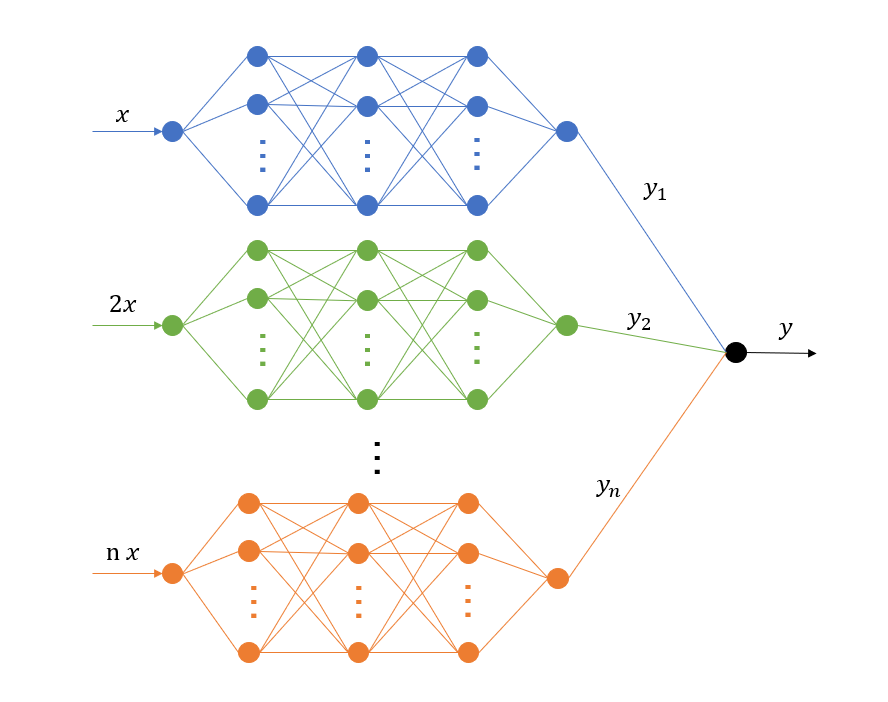
\includegraphics[width=0.5\linewidth]{MscaleNet2}
\caption{Mscale网络结构}
\label{net}
\end{figure}

\section*{代码实现细节}

代码文件说明:

\begin{itemize}
\item \textbf{ritzN.py}:用一般的Normal网络求解椭圆方程。
\item \textbf{ritzM.py}:用Mscale网络求解椭圆方程。
\item \textbf{plot\_result.py}:展示网络结果,画图。
\item \textbf{my\_act.py}:文件中定义了可能用到的激活函数,如果要用到新的激活函数可以在这里添加。\textbf{act\_dict}变量下标是激活函数的“名字”,它的值是名字对应的函数句柄。
\end{itemize}

\textbf{运行环境:python 3.6 + tensorflow 1.16}

\subsection*{参数设定}

在代码中,首先我们要设定所有的参数,以便修改。所有的参数和运行结果都记录在变量\textbf{R}中。

\begin{lstlisting}
R = {}

R["seed"] = 0

R["size_it"] = 1000
R["size_bd"] = 100

R["penalty"] = 1e3

R["act_name"] = ("sin",) * 3
R["hidden_units"] = (180,) * 3
R["learning_rate"] = 1e-4
R["lr_decay"] = 5e-7

R["varcoe"] = 0.5

R["total_step"] = 5000
R["resamp_epoch"] = 1
R["plot_epoch"] = 500

R["record_path"] = os.path.join("..", "exp", "sin_N")
\end{lstlisting}

参数意义如下:

\begin{itemize}
\item \textbf{seed}:随机数种子。保证两次运行代码的结果完全一样。(在必要的时候,这个也是可调的参数之一)
\item \textbf{size\_it}:区域$\Omega$内部随机生成的点的个数,也就是$|S_1|$。
\item \textbf{size\_bd}:区域边界$\partial \Omega$上随机生成的点的个数,也就是$|S_2|$。
\item \textbf{penalty}:惩罚系数,就是公式中的$\beta$。
\item \textbf{scale}:Mscale网络中的变换系数。(Normal网络中没有这个参数)
\item \textbf{act\_name}:长度为$N$的列表,代表每一层的激活函数。
\item \textbf{hidden\_units}:长度为$N$的列表,代表每一层的宽度。
\item \textbf{learning\_rate}:学习率。(一般不能太大)
\item \textbf{lr\_decay}:学习率下降速度。
\item \textbf{varcoe}:初始化参数。
\item \textbf{total\_step}:训练总步数。
\item \textbf{resamp\_epoch}:采样间隔。每隔X步重新随机生成$S_1,S_2$中的点。X=1代表每计算一步都重新随机生成点。X大于总步数时,代表训练用的样本不变。
\item \textbf{plot\_epoch}:从第0步开始,每隔X步记录下数值解图像。同时输出当前状态。
\item \textbf{record\_path}:保存记录的文件夹路径。在运行结束的时候,源代码文件会被复制到文件夹下的\textbf{code.py}文件中,以便重复实验。数据结果和参数会保存在文件夹下的\textbf{data.pkl}文件中,以便画图和展示。
\end{itemize}

\subsection*{定义求解区域}

这一部分定义了求解区域$\Omega$。\textbf{如果要求解复杂区域上的方程,就要修改这部分代码。}

\begin{lstlisting}
R["dimension"] = dim = 2
R["area_it"] = 4
R["area_bd"] = 8

# interior data
def rand_it(size):
    x_it = np.random.rand(size, dim) * 2 - 1
    return x_it.astype(np.float32)

# boundary data
def rand_bd(size):

    x_bd = np.random.rand(size, dim) * 2 - 1
    ind = np.random.randint(dim, size=size)
    x01 = np.random.randint(2, size=size) * 2 - 1
    for ii in range(size):
        x_bd[ii, ind[ii]] = x01[ii]
    return x_bd.astype(np.float32)
\end{lstlisting}

这里\textbf{dim}是方程的空间维数,\textbf{area\_it}表示$\Omega$的面积。\textbf{area\_bd}表示$\partial \Omega$的面积。

\textbf{rand\_it}函数,生成$\Omega$内\textbf{均匀分布}的随机点,输入需要的随机点个数\textbf{size},返回一个大小为$size \times dim$的数组。

\textbf{rand\_bd}函数,生成边界$\partial \Omega$上\textbf{均匀分布}的随机点,输入输出同上。

这样就定义了求解区域。这里对应的求解区域是$[-1,1]^2$。想要在其它区域上求解,只要重新实现一遍这个函数。

\subsection*{定义方程}

这一部分定义了方程中的已知函数$a(x),c(x),f(x)$,和精确解(边界条件)$u(x)$。如果精确解未知,$u(x)$就代表边界条件。\textbf{如果要求解其它方程,就要修改这部分代码。}

\begin{lstlisting}
# PDE problem
# - (a(x) u'(x))' + c(x) u(x) = f(x)
R["mu"] = mu = 6 * np.pi

def u(x):
    u = np.sin(mu * x)
    return u.astype(np.float32).reshape((-1, 1))

def a(x):
    a = np.ones((x.shape[0], 1))
    return a.astype(np.float32).reshape((-1, 1))

def c(x):
    c = np.zeros((x.shape[0], 1))
    return c.astype(np.float32).reshape((-1, 1))

def f(x):
    f = mu * mu * np.sin(mu * x)
    return f.astype(np.float32).reshape((-1, 1))
\end{lstlisting}

需要注意的是:这些函数,输入都是一个大小为$size \times dim$的数组,每一行代表一个采样点。返回的是大小为$size \times 1$的数组。(这里的维度不一致会报错)

\subsection*{保存参数}

把源代码文件复制到文件夹下的\textbf{code.py}文件中,以便重复实验。设定随机数种子。

\begin{lstlisting}
# save parameters

# prepare folder
if not os.path.isdir(R["record_path"]):
    os.mkdir(R["record_path"])

# save current code
save_file = os.path.join(R["record_path"], "code.py")
shutil.copyfile(__file__, save_file)

# set seed
tf.set_random_seed(R["seed"])
tf.random.set_random_seed(R["seed"])
np.random.seed(R["seed"])
\end{lstlisting}

\subsection*{用于画图和计算误差的采样点}

这里的\textbf{x\_test}是用于计算误差的采样点,\textbf{u\_test\_true}是这些点上的精确解的值。计算数值解和精确解误差的时候就在这些点上计算。

\textbf{x\_samp}是用于画图的采样点。\textbf{u\_samp\_true}是这些点上的精确解的值。

\textbf{如果我们不知道精确解,而是通过差分方法或者其它方法生成的参考解。这里的\textbf{u\_test\_true}就要从文件里面读取出来。}

\begin{lstlisting}
# get test points
x_test = np.linspace(-1, 1, 200 +1).reshape((-1, 1))

R["x_test"] = x_test.astype(np.float32)
R["u_test_true"] = u(R["x_test"])

# get sample points
x_samp = np.linspace(-1, 1, 200 +1).reshape((-1, 1))

R["x_samp"] = x_samp.astype(np.float32)
R["u_samp_true"] = u(R["x_samp"])
\end{lstlisting}

需要注意的是:这里的\textbf{x\_test}和\textbf{x\_samp}都是$size \times dim$的数组,每一行代表一个采样点。这里的\textbf{u\_test\_true}和\textbf{u\_samp\_true}都是$size \times 1$的数组。在画图时要另外调整。

之后在训练的过程中,还会有\textbf{u\_test\_X}和\textbf{u\_samp\_X}变量,代表训练到第X步的数值解。

\subsection*{神经网络}

用tensorflow实现深度学习的网络结构。

\textbf{如果要换网络结构或者参数初始化,就要改这段代码。}

下面这段代码实现了一个普通的网络(Normal),\textbf{init\_W}和\textbf{init\_b}是变量的初始值。

\begin{lstlisting}
units = (dim,) + R["hidden_units"] + (1,)

def neural_net(x):
    with tf.variable_scope("vscope", reuse=tf.AUTO_REUSE):

        y = x

        for i in range(len(units) - 2):
            init_W = np.random.randn(units[i], units[i + 1]).astype(np.float32)
            init_W = init_W * (2 / (units[i] + units[i + 1]) ** R["varcoe"])
            init_b = np.random.randn(units[i + 1]).astype(np.float32)
            init_b = init_b * (2 / (units[i] + units[i + 1]) ** R["varcoe"])

            W = tf.get_variable(name="W" + str(i), initializer=init_W)
            b = tf.get_variable(name="b" + str(i), initializer=init_b)

            y = act_dict[R["act_name"][i]](tf.matmul(y, W) + b)

        init_W = np.random.randn(units[-2], units[-1]).astype(np.float32)
        init_W = init_W * (2 / (units[i] + units[i + 1]) ** R["varcoe"])
        init_b = np.random.randn(units[-1]).astype(np.float32)
        init_b = init_b * (2 / (units[i] + units[i + 1]) ** R["varcoe"])

        W = tf.get_variable(name="W" + str(len(units) - 1), initializer=init_W)
        b = tf.get_variable(name="b" + str(len(units) - 1), initializer=init_b)

        y = tf.matmul(y, W) + b

    return y
\end{lstlisting}

下面这段代码实现了Mscale网络,原理类似。

\begin{lstlisting}
units = (dim,) + R["hidden_units"] + (1,)

def neural_net(x):
    with tf.variable_scope("vscope", reuse=tf.AUTO_REUSE):

        all_y = []
        for k in range(len(R["scale"])):
            scale_y = R["scale"][k] * x

            for i in range(len(units) - 2):
                init_W = np.random.randn(units[i], units[i + 1]).astype(np.float32)
                init_W = init_W * (2 / (units[i] + units[i + 1]) ** R["varcoe"])
                init_b = np.random.randn(units[i + 1]).astype(np.float32)
                init_b = init_b * (2 / (units[i] + units[i + 1]) ** R["varcoe"])

                W = tf.get_variable(name="W" + str(i) + str(k),
                    initializer=init_W)
                b = tf.get_variable(name="b" + str(i) + str(k),
                    initializer=init_b)

                scale_y = act_dict[R["act_name"][i]](tf.matmul(scale_y, W) + b)

            init_W = np.random.randn(units[-2], units[-1]).astype(np.float32)
            init_W = init_W * (2 / (units[i] + units[i + 1]) ** R["varcoe"])
            init_b = np.random.randn(units[-1]).astype(np.float32)
            init_b = init_b * (2 / (units[i] + units[i + 1]) ** R["varcoe"])

            W = tf.get_variable(name="W" + str(len(units) - 1) + str(k),
                initializer=init_W)
            b = tf.get_variable(name="b" + str(len(units) - 1) + str(k),
                initializer=init_b)

            scale_y = tf.matmul(scale_y, W) + b

            all_y.append(scale_y)

        y = sum(all_y)

    return y
\end{lstlisting}

\subsection*{损失函数}

定义损失函数。这里变量前面的“V”代表它的类型是tensorflow中的Variable,变量前面的“N”表示它保存变量当前的取值。

\textbf{如果求解的不是椭圆方程,或者损失函数的形式有变化,就要改这段代码。}

\begin{lstlisting}
# loss and optimizer ("V" for variable)
with tf.variable_scope("vscope", reuse=tf.AUTO_REUSE):

    Vx_it = tf.placeholder(tf.float32, shape=(None, dim))
    Vx_bd = tf.placeholder(tf.float32, shape=(None, dim))

    Va_it = tf.placeholder(tf.float32, shape=(None, 1))
    Vc_it = tf.placeholder(tf.float32, shape=(None, 1))
    Vf_it = tf.placeholder(tf.float32, shape=(None, 1))

    Vu_true_bd = tf.placeholder(tf.float32, shape=(None, 1))

    Vu_it = neural_net(Vx_it)
    Vu_bd = neural_net(Vx_bd)

    Vdu_it = tf.gradients(Vu_it, Vx_it)[0]

    Vloss_it = R["area_it"] * tf.reduce_mean(
        1 / 2 * Va_it * tf.reduce_sum(tf.square(Vdu_it), axis=1, keepdims=True)
      + 1 / 2 * Vc_it * tf.square(Vu_it)
      - Vf_it * Vu_it
    )
    Vloss_bd = R["area_bd"] * tf.reduce_mean(tf.square(Vu_bd - Vu_true_bd))

    Vloss = Vloss_it + R["penalty"] * Vloss_bd

    learning_rate = tf.placeholder_with_default(input=1e-3, shape=[], name="lr")
    optimizer = tf.train.AdamOptimizer(learning_rate)
    train_op = optimizer.minimize(Vloss)
\end{lstlisting}

\subsection*{开始训练}

\textbf{这里的代码一般不用大改,但是如果前面有改动,这里的要和之前的匹配。}

随机生成定义域里的点,计算这些点上的函数值。
\begin{lstlisting}
# generate new data ("N" for number)
if epoch % R["resamp_epoch"] == 0:
    Nx_it = rand_it(R["size_it"])
    Nx_bd = rand_bd(R["size_bd"])
    Na_it = a(Nx_it)
    Nc_it = c(Nx_it)
    Nf_it = f(Nx_it)
    Nu_bd = u(Nx_bd)
\end{lstlisting}

把生成的数据喂给网络,训练一步。
\begin{lstlisting}
_, Nloss, Nloss_bd = sess.run(
    [train_op, Vloss, Vloss_bd],
    feed_dict={
        Vx_it: Nx_it,
        Vx_bd: Nx_bd,
        Va_it: Na_it,
        Vc_it: Nc_it,
        Vf_it: Nf_it,
        Vu_true_bd: Nu_bd,
        learning_rate: lr,
    },
)
\end{lstlisting}

代入采样点,计算数值解和真实解之间的误差
\begin{lstlisting}
R["u_test"] = sess.run(Vu_it, feed_dict={Vx_it: R["x_test"]})
Nerror = R["area_it"] * np.mean((R["u_test"] - R["u_test_true"]) ** 2)
\end{lstlisting}

每过\textbf{plot\_epoch}步,记录下当时的数值解,同时输出当前误差。
\begin{lstlisting}
if epoch % R["plot_epoch"] == 0:
    print("epoch %d, time %.3f" % (epoch, time.time() - t0))
    print("total loss %f, boundary loss %f" % (Nloss, Nloss_bd))
    print("interior error %f" % (Nerror))

    u_samp = sess.run(Vu_it, feed_dict={Vx_it: R["x_samp"]})
    R["u_samp_" + str(epoch)] = u_samp
\end{lstlisting}

最后保存所有参数
\begin{lstlisting}
# save data
data_dir = os.path.join(R["record_path"], "data.pkl")
with open(data_dir, "wb") as file:
    pickle.dump(R, file)
\end{lstlisting}

\section*{测试用例}

具体参数如上,分别用规模为(180,180,180)的普通全连接网络(Normal),系数为(1,2,4,8,16,32)的6个规模为(30,30,30)的网络(Mscale),和系数全是32的6个规模为(30,30,30)的网络(Noscale)求解方程。激活函数为sin(x).

方程的精确解为$u = \sin 6 \pi x$。

(mscale1-32)求解过程中,数值解随训练的变化如图\ref{proc}。蓝色实线是精确解,红色虚线是数值解。
\begin{figure}[h]
\centering
\subfloat[0步]{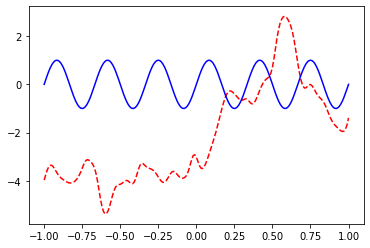
\includegraphics[width=0.24\linewidth]{s0}}
\subfloat[500步]{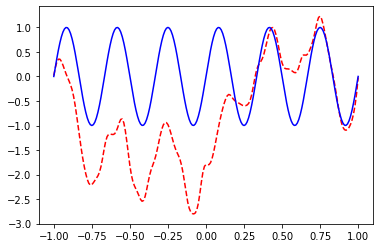
\includegraphics[width=0.24\linewidth]{s500}}
\subfloat[1000步]{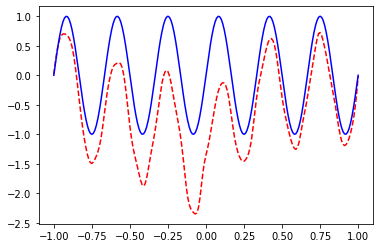
\includegraphics[width=0.24\linewidth]{s1000}}
\subfloat[5000步]{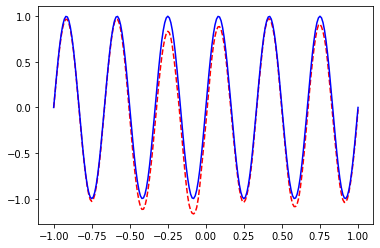
\includegraphics[width=0.24\linewidth]{s5000}}
\caption{求解过程}
\label{proc}
\end{figure}

三种方法error下降对比如图\ref{error}。横轴是训练步数,纵轴是测试误差。
\begin{figure}[h]
\centering
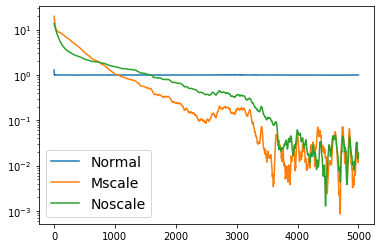
\includegraphics[width=0.3\linewidth]{error}
\caption{误差下降曲线}
\label{error}
\end{figure}

\begin{thebibliography}{99}  
\bibitem{deep-ritz} Weinan E ,Yu B. The Deep Ritz method: A deep learning-based numerical algorithm for solving variational problems[J]. Communications in Mathematics \& Stats, 2018, 6(1):1-12.
\bibitem{mscale}Ziqi Liu,Wei Cai,Zhi-Qin John Xu. Multi-scale Deep Neural Network (MscaleDNN) for Solving Poisson-Boltzmann Equation in Complex Domains[J]. 2020. arXiv:2007.11207 [physics.comp-ph]
\end{thebibliography}

\end{document}
